


% svg debiliškai gaunas, sueis screeshot'as for the moment
% redaguoti galima čia https://demo.bpmn.io/s/start
% originalus failas: processes.bpmn

\begin{landscape}
\section{Procesų aprašymas}
Dokumente pateiktos diagramos sumodeliuotos naudojant BPMN 2.0 notaciją.
\thispagestyle{empty}
\begin{figure}[H]%[htpb!]
    \centering
    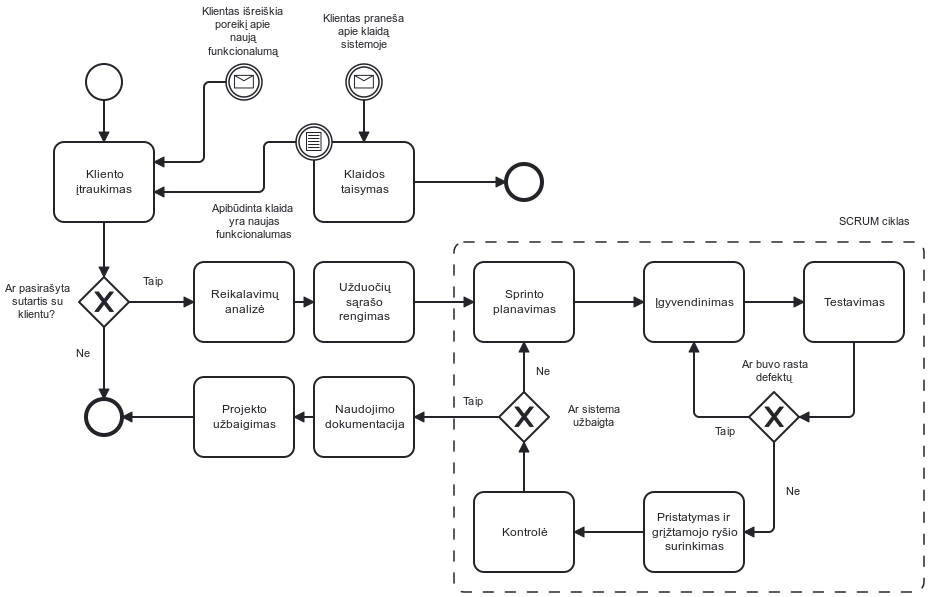
\includegraphics[width=0.85\linewidth]{task-1/etc/diagrams/processes.png}
\end{figure}
\end{landscape}

\subsection{\process{EngageClient}} % ARNAS

\begin{figure}[H]%[htpb!]
    \centering
    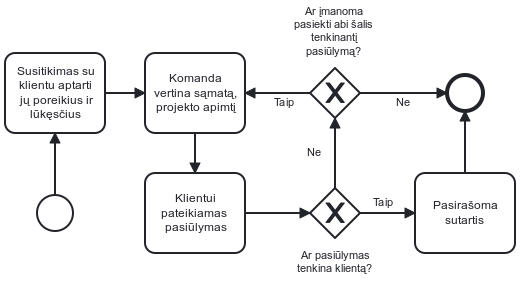
\includegraphics[width=0.75\linewidth]{task-1/etc/diagrams/engage-client.png}
\end{figure}

\begin{processTable}{EngageClient}
    \tikslas{Siekiama įvertinti kliento poreikius, rasti kompromisą dėl projekto sąmatos bei apimties ir pasirašyti sutartį.}
    \inputs{

        \item \workProd{ClientNeeds} (šis darbo produktas yra išorinis)
        
        \item \workProd{Experience}
    }
    \outputs{   
        \item \workProd{ResourceEstimates}
        
        \item \workProd{ProjectScope}
        
        \item \workProd{Contract}
    }
    \veiklos{
         \item Projektų vadovas, architektas ir analitikas bendrauja su klientu, aiškinasi jo poreikius projektui (\workProdId{ClientNeeds}). Ši veikla tęsiasi tol, kol įmonės atstovai surenka pakankamai informacijos paruošti klientui pasiūlymą.
    
        \item Projektų vadovas, architektas ir analitikas tarpusavyje įvertina kliento poreikius projektui (\workProdId{ClientNeeds}) atsižvelgdami į departamento patirtį su kitais projektais (\workProdId{Experience}) ir nustato laiko, kainos ir žmogiškųjų ištekliu sąmata (\workProdId{ResourceEstimates}) bei projekto apimtį (\workProdId{ProjectScope}). Laikas, kaina (nustatyti iš \workProdId{ResourceEstimates}), projekto apimtis (\workProdId{ProjectScope}), produkto perdavimo sąlygos ir adaptacinio laikotarpio terminas tuomet yra teisiškai įforminami sutartyje (\workProdId{Contract}). \label{activity:prepare-deal}

        \item Klientui yra pateikiama sutartis (\workProdId{Contract}). Jei klientas yra patenkintas sutarties sąlygomis, pereinama prie sutarties pasirašymo \ref{activity:sign}. Klientas gali nesutikti su sutarties sąlygomis. Tokiu atveju vyksta derybos - klientas pateikia naujus poreikius (\workProdId{ClientNeeds}) ir dar kartą vykdoma veikla \ref{activity:prepare-deal}. Jei abi šalys nesugeba rasti kompromiso, procesas gali būti nutrauktas ir darbas su klientu netęsiamas.

        \item Pasirašoma sutartis su klientu (\workProdId{Contract}). \label{activity:sign}
    }
\end{processTable}

\newpage
\subsection{\process{RA}} % DOMANTAS

\begin{processTable}{RA}
    \tikslas{
    Išskirti funkcinius ir nefunkcinius reikalavimus, apibrėžti aukšto lygio architektūrą.
    }
    \inputs{
        \item \workProd{ProjectScope}
        \item \workProd{Contract}
    }
    \outputs{
        \item \workProd{FunReq}
        \item \workProd{NonFunReq}
        \item \workProd{HighLevelArch}
    }
    \veiklos{
        \item Analitikas renka informaciją iš kliento. Pagal tai modeliuoja verslo procesus ir identifikuoja konkrečius naudotojų poreikius.
        \item Architektas ir analitikas apibrėžia funkcinius (\workProdId{FunReq}) ir nefunkcinius reikalavimus (\workProdId{NonFunReq}) iš
            \begin{itemize}
                \item identifikuotų naudotojų poreikių
                \item modeliuojamų verslo procesų
                \item projekto apimties (\workProdId{ProjectScope})
            \end{itemize}
        \item Architektas sukuria aukšto lygio sistemos architektūrą (\workProdId{HighLevelArch}) atsižvelgdamas į apibrėžtus funkcinius (\workProdId{FunReq}) ir nefunkcinius reikalavimus (\workProdId{NonFunReq}).
    }
\end{processTable}

\newpage
\subsection{\process{DraftBacklog}} % ARNAS

\begin{processTable}{DraftBacklog}
    \tikslas{Iš reikalavimų analizės rezultatų sudaryti projekto užduočių sąrašą.}
    
    \inputs{
        \item \workProd{FunReq}
        \item \workProd{NonFunReq}
        \item \workProd{HighLevelArch}
    }
    
    \outputs{
        \item \workProd{Backlog}
    }
    
    \veiklos{

        \item Architektas kartu su analitiku grupuoja susijusius funkcinius (\workProdId{FunReq}) ir nefunkcinius (\workProdId{NonFunReq}) reikalavimus bei skaido aukšto lygio architektūrą (\workProdId{HighLevelArch}) į panaudos atvejus arba bendro pobūdžio užduotis, kurios bendrai sudaro projekto užduočių sąrašą (\workProdId{Backlog}).

        \item Architektas kartu su analitiku detaliai aprašo užduotis, nurodydami kokie funkciniai (\workProdId{FunReq}) bei nefunkciniai (\workProdId{NonFunReq}) reikalavimai įeiną į konkrečios užduoties apimtį.
        \item Architektas kartu su analitiku nurodo užduočių priėmimo kriterijus, kuriais vadovaujantis galima  objektyviai įvertini ar užduotis yra įgyvendinta.
        \item Projektų vadovas, architektas ir analitikas prioritetizuoja projekto užduočių sąrašą (\workProdId{Backlog}) jį surūšiuodami.
    }
\end{processTable}

\newpage
\subsection{\process{ScrumCycle}}

%  ## Domanto klausimai
% 
%  - Jeigu sprinto backlog'e įdedamos klaidos (t.y. klaida yra tiesiog dar vienas task'as sprinto užduočių sąraše), kam tada reikalingas "KL. Klaidos" darbo produktas?

\subsubsection{\process{Refinement}}

\begin{processTable}{Refinement}
    \tikslas{
        Sudaryti sprinto užduočių sąrašą.
    }
    \inputs{
        \item \workProd{Backlog}
        \item \workProd{SprintReviewDoc} (tik nuo antro sprinto)
        \item \workProd{StoryPointRange} (tik nuo antro sprinto)
    }
    \outputs{
        \item \workProd{SprintBacklog}
        \item \workProd{Backlog}
    }
    \veiklos{
        \item Projektų vadovas, kuris atsižvelgia į sprinto peržiūros ataskaitą (\workProdId{SprintReviewDoc}), nustato sprinto tikslus. Jei istoriniai praėjusių sprintų duomenys dar neegzistuoja, nes vykdomas pirmasis sprintas, atsižvelgiama į projektų užduočių sąrašo (\workProdId{Backlog}) pirminę prioritetizacija.
        \label{SP:1}

        \item Projektų vadovas, bendro komandos susitikimo metu, \ref{SP:1}  veikloje įvardintus tikslus paskelbia komandai. Į tai atsižvelgę komandos nariai gali atnaujinti projekto užduočių sąrašo (\workProdId{Backlog}) prioritetus.
        \item Jei komandos nariai nusprendžia, kad tam tikra užduotis iš projekto užduočių sąrašo (\workProdId{Backlog})  turi būti išskaidoma į atomiškas užduotis, tai ir yra atliekama - skaidomai užduočiai sukuriamos vaikinės užduotys.
        \item Komanda kiekvienai neįvertintai užduočiai įvertina laiką ir pastangas, naudojant pasakojimo vienetus, įprastai sekančius Fibonači seką.  Tai atliekama remiantis kelių komandos narių darbine patirtimi ir bendru susitarimu. Tuomet projekto užduočių sąraše (\workProdId{Backlog}) esančios užduoties atributas -- pasakojimo vienetai -- keičiamas į nutartą skaičių.
        \item Projektų vadovas sukuria sprinto užduočių sarašą (\workProdId{SprintBacklog}) atrinkdamas aukščiausio prioriteto  užduotis iš projekto užduočių sąrašo (\workProdId{Backlog})  taip, kad jų bendra pasakojimo vienetų suma tilptų į pasakojimo vienetų intervalą (\workProdId{StoryPointRange}). Pirmojo sprinto metu, dar neturint pasakojimo vienetų intervalo, parenkama tiek užduočių, kiek komanda bendru nutarimu nusprendžia.
        \item Komandos nariai planuoja, kas atliks kurią sprinto užduotį. Nutarus, sprinto užduočių sąraše (\workProdId{SprintBacklog}) kiekvienos užduoties atributas -- atsakingas asmuo --  keičiamas į už užduoties įgyvendinimą atsakingo asmens vardą ir pavardę.
    }
\end{processTable}

\newpage
\subsubsection{\process{Development}}

\begin{processTable}{Development}
    \tikslas{
         Atlikti sprinto užduočių sąraše išvardytas užduotis.
    }
    \inputs{
        \item \workProd{SprintBacklog}
        \item \workProd{DefectReport}
        \item \workProd{Codebase}
        \item \workProd{TechDoc}
    }
    \outputs{
        \item \workProd{SprintBacklog}
        \item \workProd{Codebase}
        \item \workProd{TechDoc}
    }
    \veiklos{
        \item Kai programinės įrangos kūrėjai atlieka jiems priskirtą užduotį, užduoties statusas keičiamas IN PROGRESS. 
        \item Jei šis procesas vykdomas, kai užduotis buvo grąžinta į įgyvendinimą (\textit{ĮG}) po testavimo proceso (\textit{TE}), programinės įrangos kūrėjai atsižvelgia į klaidų aprašus (\workProdId{DefectReport}), kad ištaisytų klaidas. Kitu atveju veikla praleidžiama.
        \label{IG:2}
        \item Kiekvienas programinės įrangos kūrėjas rašo kodą, taip papildydami programinį kodą   
        (\workProdId{Codebase}). 
        \label{IG:3}
        \item Programinės įrangos kūrėjai rašo vienetų testus, kurie padengia 70\% kodo eilučių, kad užtikrintų kodo korektiškumą. Laikoma, kad yra atnaujinamas programinis kodas (\workProdId{Codebase}).
        \label{IG:4}
        \item Programinės įrangos kūrėjas, atsakingas už užduotį, keičia užduoties statuso atributą į \mbox{IN~REVIEW}.
        \label{IG:5}
        \item Užduotį, kuri yra IN REVIEW, kitas komandos narys peržiūri, komentuoja kodą. Jeigu kitas komandos narys pareikalauja pakeitimų, pakeičia užduoties statusą į IN PROGRESS. Už užduotį atsakingas asmuo turi pakartoti \ref{IG:3}-\ref{IG:6} veiklas.
        \label{IG:6}
        \item Kitam komandos nariui patvirtinus kodo kokybę, programinės įrangos kūrėjas pažymi, kad programinį kodą (\workProdId{Codebase}) galima testuoti - užduoties statusas keičiamas į TESTING, o atributas atsakingas asmuo  keičiamas į už užduoties testavimą atsakingo asmens vardą ir pavardę.  
        \label{IG:7}
        \item Visą reikalingą techninę dokumentaciją (\workProdId{TechDoc}) parašo programinės įrangos kūrėjas.
        \label{IG:8}
        \item Laikas, praleistas atliekant \ref{IG:2}-\ref{IG:8} veiklas pažymimas sprinto užduočių sąrašo (\workProdId{SprintBacklog})  užduoties atribute  „kūrimo valandos“.
    }
\end{processTable}

\newpage
\subsubsection{\process{Testing}}

\begin{processTable}{Testing}
    \tikslas{
        Verifikuoti programinį kodą.
    }
    \inputs{
        \item \workProd{SprintBacklog}
        \item \workProd{DefectReport} (nuo antro sprinto)
        \item \workProd{Codebase}
        \item \workProd{TechDoc}
    }
    \outputs{
        \item \workProd{DefectReport}
        \item \workProd{SprintBacklog}
        \item \workProd{Codebase}
    }
    \veiklos{
        \item Kiekvienas testuotojas atlieka jam priskirtą užduotį kaip nurodyta sprinto užduočių saraše (\workProdId{SprintBacklog}). 
        \label{TE:1}
        \item Testuotojai testuoja užduoties programinį kodą (\workProdId{Codebase}) pagal užduoties aprašymą, kuriame nurodyti funkciniai ir nefunkciniai reikalavimai. Jie taip pat atsižvelgia į užduoties priėmimo kriterijus, kurie nurodyti viename iš užduoties atributų. Pagal patirtį arba pasitarę su kitais komandos nariais, testuotojai gali nuspręsti atlikti integracijos, našumo, saugumo, regresijos ir kitus testus. 
        \label{TE:2}
        \item Testuotojai rašo arba taiso klaidų aprašus (\workProdId{DefectReport}), kad jie atspindėtų programinio kodo kokybės būklę.
         \label{TE:3}
        \item Jei šio proceso metu buvo rasta klaidų, užduotis grąžinama atgal į įgyvendinimo (\processId{Development}) procesą, kad programinės įrangos kūrėjai išspręstų klaidas. Testuotojas turi pakeisti užduoties būseną, kad sprinto užduočių sąraše (\workProdId{SprintBacklog}) būtų nurodyta, kad jos statusas IN PROGRESS, o atributas -- atsakingas asmuo -- keičiamas į už užduoties taisymą atsakingo asmens vardą ir pavardę.  
         \label{TE:4}
        \item Laikas, kuris buvo praleistas atliekant \ref{TE:2}-\ref{TE:4} veiklas pažymimas sprinto užduočių sąraše (\workProdId{SprintBacklog}) esančios užduoties atribute 
         „testavimo valandos“.
    }
\end{processTable}

\newpage
\subsubsection{\process{PartialDelivery}}

\begin{processTable}{PartialDelivery}
    \tikslas{
       Pristatyti suinteresuotoms šalims atliktą darbą ir surinkti grįžtamąjį ryšį.
    }

    \inputs{
        \item \workProd{Codebase}
        \item \workProd{Backlog}
    }
    \outputs{
       \item \workProd{Feedback}
       \item \workProd{Product}
    }
    \veiklos{
        \item Programinės įrangos kurėjai sukuria naujos produkto versijos (\workProdId{Product}) artefaktą.
        \item Programinės įrangos kūrėjas pristato produktą (\workProdId{Product}) suinteresuotoms šalims.
        \item Komandos nariai išklauso SŠ atsiliepimus apie atliktą darbą. Aptaria visus trūkumus, galimus patobulinimus ir pakeitimus projekto užduočių sąraše (\workProdId{Backlog}).
        \item Projekto vadovas surašo surinktus atsiliepimus į grįžtamojo ryšio registrą (\workProdId{Feedback}).
    }
\end{processTable}

\newpage
\subsubsection{\process{Control}}

\begin{processTable}{Control}
    \tikslas{
        Įvertinti kaip sekėsi sprintas ir suderinti būsimų scrum ciklų patobulinimus.
    }
    \inputs{
        \item \workProd{DefectReport}
        \item \workProd{SprintBacklog}
        \item \workProd{ResourceEstimates}
        \item \workProd{StoryPointRange}
        \item \workProd{Feedback}
        \item \workProd{Backlog}
    }
    \outputs{
        \item \workProd{SprintReviewDoc}
        \item \workProd{StoryPointRange}
    }
    \veiklos{
        \item Visi komandos nariai apmąsto sprinto eigą, aptaria, kas pavyko ir su kokiais sunkumais susidūrė. Visi komandos nariai surašo savo  atsiliepimus.
        
        \item Projekto vadovas peržiūri sprinto užduočių sąrašą (\workProdId{SprintBacklog}), palygina faktinį užduotims atlikti sugaištą laiką su kūrimo valandų įvertinimais ir parengia laiko valdymo ataskaitą atsižvelgdamas į likusį laiką iš pradinių sąmatų (\workProdId{ResourceEstimates}).

        \item Remiantis grįžtamojo ryšio registru (\workProdId{Feedback}) ir laiko valdymo ataskaita, projekto vadovas atlieka projekto užduočių sąrašo (\workProdId{Backlog}) atnaujinimą, prireikus, užduočių prioritetų keitimą, pasakojimo vienetų intervalo (\workProdId{StoryPointRange}) patikslinimą. Šie pakeitimai fiksuojami sprinto peržiūros ataskaitoje (\workProdId{SprintReviewDoc}).
        
        \item Remiantis komandos atsiliepimais, komanda ir projektų vadovas nustato komandos procesų pakeitimus, kurie įsigalioja nuo kito sprinto.
        % \item Based on \textbf{1-2} and feedback documentation (\textit{FD}), the project manager and scrum team identifies necessary adjustments for the next sprint.
        
        % NOTE: Bet ar tai tikrai reikia čia atlikti? Gal geriau tai pažymėti sprinto peržiūros ataskaitoj ir td koregavimas atliekamas Sprinto Planavime?? also jeigu keičiama čia, tai reikia pridėti atitinkamai prie input'ų ir output'ų.
        
        % This includes updating the project backlog (\textit{PB}), reprioritizing tasks as needed and capturing these changes in the sprint review report (\textit{SRR}), refining the story point range (\textit{SP}).

        \item Jei projekto užduočių sąraše (\workProdId{Backlog}) visų užduočių statusas yra DONE, pereinama prie naudojimo dokumentacijos (\processId{CreateManual}), o SCRUM ciklai šiam projektui nebetęsiami.
        % NOTE: čia gal nurodyti kokiomis sąlygomis nebereikia kitų sprint'ų?
        % \item The project manager closes project if necessary - if no further sprints are required, they transition to usage documentation.
    }
\end{processTable}

\newpage
\subsection{\process{CreateManual}}

\begin{processTable}{CreateManual}
    \tikslas{Paruošti produkto naudojimo instrukciją, suprantamą naudotojams.}
    \inputs{
        \item \workProd{Backlog}
        \item \workProd{Product}
    }
    \outputs{
            \item \workProd{Manual}
    }
    \veiklos{
        \item Iš užduočių sąrašo (\workProdId{Backlog}) išrenkami panaudos atvejai. 
        \item Detaliai aprašomi visi žingsniai kiekvienam panaudos atvejui įgyvendinti naudojant produkto (\workProdId{Product}) iliustracijas. \label{CreateManual/1}
        \item Detaliai aprašomos visos produkto (\workProdId{Product}) funkcijos (t.\,y. kaip jomis pasinaudoti). \label{CreateManual/2}
        \item Iš \ref{CreateManual/1} ir \ref{CreateManual/2} veiklų rezultatų sudaromas struktūrizuotas, vientisas dokumentas - \prodWork{Manual}
        \item Atliekama produkto naudojimo instrukcijos (\workProdId{Manual}) validacija - paruoštas dokumentas peržiūrimas kolegų iš kitų padalinių, įsitikinama, jog instrukcija suprantama pirmą kartą produktą (\workProdId{Product}) naudojantiems žmonėms. \label{CreateManual/3}
        \item Kol netenkinamas \ref{CreateManual/3} punktas, atliekami naudojimo instrukcijos pakeitimai.
        }
\end{processTable}

\begin{figure}[!h]
    \centering
    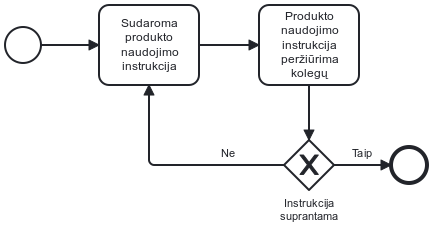
\includegraphics[width=0.75\linewidth]{task-1/etc/diagrams/Manual.png}
\end{figure}
% --------------------------------------------------------------------
\newpage
\subsection{\process{CloseProject}}
\begin{processTable}{CloseProject}
    \tikslas{Užbaigti projektą, perduoti paruoštą naudojimui produktą klientams.}
    \inputs{
        \item \workProd{Product}
    	\item \workProd{Contract}
    	\item \workProd{Backlog}
    	\item \workProd{TechDoc}
    	\item \workProd{Manual}
    }
    \outputs{
        \item \workProd{Warranty}
        \item \workProd{Experience}
    }
    \veiklos{
        \item Atliekami sutartyje (\workProdId{Contract}) numatyti produkto (\workProdId{Product}) perdavimo klientui darbai.
        \item Klientui perduodama \prodWork{Manual}.
        \item Klientui perduodama \prodWork{TechDoc}.
        \item Sudaroma ir pasirašoma \prodWork{Warranty}, kurioje numatomas garantinio aptarnavimo laikotarpis.
    	\item Atliekama vidinė komunikacija apie užbaigtą projektą. Projekto vadovas dalinasi projekto eiga, priimtais kritiniais sprendimais ir rezultatais. Taip kaupiama \prodWork{Experience}. 
    	\item Kol nesibaigia sutartyje (\workProdId{Contract}) numatytas adaptacinis laikotarpis, klientams teikiama techninė pagalba.
    }
\end{processTable}

\begin{figure}[!h]
    \centering
    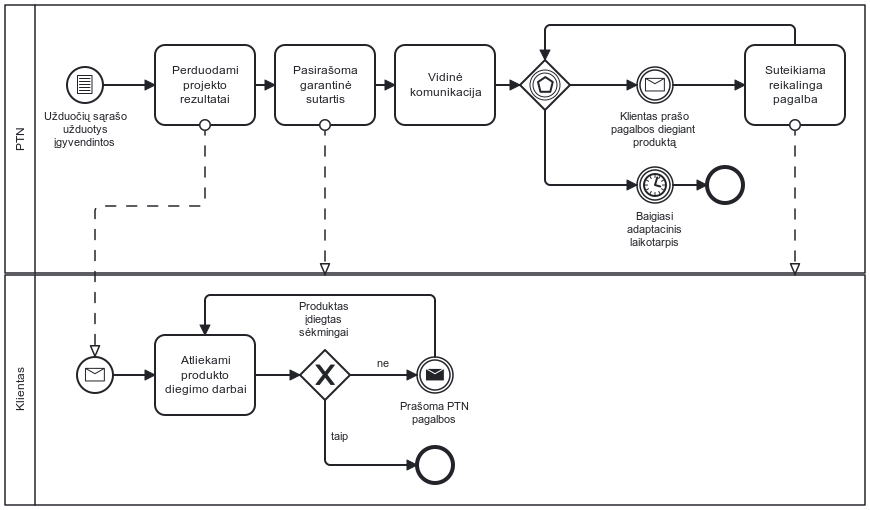
\includegraphics[width=0.8\linewidth]{task-1/etc/diagrams/projectClosure.png}
\end{figure}
\newpage

%----------------------------------------


\subsection{\process{BugFix}}
\begin{processTable}{BugFix}
    \tikslas{Ištaisyti ne dėl kliento kaltės kilusias produkto klaidas.}
    \inputs{
        \item \workProd{Product}
    	\item \workProd{TechDoc}
    	\item \workProd{Contract}
    	\item \workProd{Warranty}
    	\item \workProd{Ticket} (išorinis darbo produktas)
    	\item \workProd{Manual}
     }
    \outputs{
        \item \workProd{Ticket}
        \item \workProd{Product}
    }
    \veiklos{
        \item Atliekama pirminė užregistruotos klaidos (\workProdId{Ticket}) analizė.
	   \item Jei užregistruota klaida (\workProdId{Ticket}):
            \begin{enumerate}[label=\alph*)] 
        		\item kyla dėl produkto (\workProdId{Product}) naudojimo nesilaikant produkto naudojimo instrukcijos (\workProdId{Manual})
        		\item kyla eksploatuojant produktą (\workProdId{Product}) netinkamomis, t.\,y. neatitinkančiomis techninės dokumentacijos (\workProdId{TechDoc}), sąlygomis
        		\item yra ne klaida, o neegzistuojančio ir sutartyje (\workProdId{Contract}) nenumatyto funkcionalumo įgyvendinimo prašymas
        		\item neatitinka garantino aptarnavimo sutartyje (\workProdId{Warranty}) numatytų sąlygų
        		\item yra užregistruota po garantino aptarnavimo sutartyje (\workProdId{Warranty}) numatyto garantinio laikotarpio
            \end{enumerate}
            tuomet užregistruota klaida (\workProdId{Ticket}) nėra taisoma ir šis procesas (\processId{BugFix}) yra užbaigiamas nevykdant tolesnių veiklų.
    	\item Atliekama klaidos kilimo priežasties analizė (root cause analysis).
    	\item Kuo įmanoma greičiau ištaisoma klaida ir sukuriama nauja produkto (\workProdId{Product}) versija.
    	\item Nauja produkto (\workProdId{Product}) versija perduodama klientams.
    	\item Užregistruota klaida (\workProdId{Ticket}) „Jira“ platformoje papildoma su klaidą ištaisančia prdoukto (\workProdId{Product}) versija bei klaidos kilimo priežastimi.    
    }
\end{processTable}
\newpage

%----------------------------------------

% \begin{processTable}{PrimaryKey}
%     \tikslas{}
%     \inputs{
%        \item \workProd{Kazkas}
%     }
%     \outputs{
%        \item \workProd{Kazkas}
%     }
%     \veiklos{
%         \item Kazkokia veikla
%     }
% \end{processTable}


%----------------------------------------